% mnras_template.tex 
%
% LaTeX template for creating an MNRAS paper
%
% v3.0 released 14 May 2015
% (version numbers match those of mnras.cls)
%
% Copyright (C) Royal Astronomical Society 2015
% Authors:
% Keith T. Smith (Royal Astronomical Society)

% Change log
%
% v3.0 May 2015
%    Renamed to match the new package name
%    Version number matches mnras.cls
%    A few minor tweaks to wording
% v1.0 September 2013
%    Beta testing only - never publicly released
%    First version: a simple (ish) template for creating an MNRAS paper

%%%%%%%%%%%%%%%%%%%%%%%%%%%%%%%%%%%%%%%%%%%%%%%%%%
% Basic setup. Most papers should leave these options alone.
\documentclass[letters,usenatbib,times]{mnras}

% MNRAS is set in Times font. If you don't have this installed (most LaTeX
% installations will be fine) or prefer the old Computer Modern fonts, comment
% out the following line
\usepackage{newtxtext,newtxmath}
% Depending on your LaTeX fonts installation, you might get better results with one of these:
%\usepackage{mathptmx}
%\usepackage{txfonts}

% Use vector fonts, so it zooms properly in on-screen viewing software
% Don't change these lines unless you know what you are doing
\usepackage[T1]{fontenc}

% Allow "Thomas van Noord" and "Simon de Laguarde" and alike to be sorted by "N" and "L" etc. in the bibliography.
% Write the name in the bibliography as "\VAN{Noord}{Van}{van} Noord, Thomas"
\DeclareRobustCommand{\VAN}[3]{#2}
\let\VANthebibliography\thebibliography
\def\thebibliography{\DeclareRobustCommand{\VAN}[3]{##3}\VANthebibliography}


%%%%% AUTHORS - PLACE YOUR OWN PACKAGES HERE %%%%%

% Only include extra packages if you really need them. Common packages are:
\usepackage{graphicx}	% Including figure files
\usepackage{amsmath}	% Advanced maths commands
%% \usepackage{amssymb}	% Extra maths symbols
\usepackage{soul}
\usepackage{xcolor}  
\newcommand{\phil}[1]{\colorbox{yellow}{\bf #1}}

%%%%%%%%%%%%%%%%%%%%%%%%%%%%%%%%%%%%%%%%%%%%%%%%%%

%%%%% AUTHORS - PLACE YOUR OWN COMMANDS HERE %%%%%

% Please keep new commands to a minimum, and use \newcommand not \def to avoid
% overwriting existing commands. Example:
%\newcommand{\pcm}{\,cm$^{-2}$}	% per cm-squared

%%%%%%%%%%%%%%%%%%%%%%%%%%%%%%%%%%%%%%%%%%%%%%%%%%

%%%%%%%%%%%%%%%%%%% TITLE PAGE %%%%%%%%%%%%%%%%%%%

% Title of the paper, and the short title which is used in the headers.
% Keep the title short and informative.

\title[High-resolution ALMA observations of V4046\,Sgr]{High-resolution ALMA observations of V4046\,Sgr: a circumbinary disc with a thin ring}

% The list of authors, and the short list which is used in the headers.
% If you need two or more lines of authors, add an extra line using \newauthor
\author[R. Martinez Brunner et al.]{
Rafael Martinez-Brunner,$^{1}$\thanks{E-mail: rmartinezbrunner@gmail.com}
Simon Casassus,$^{1}$
Sebasti\'an P\'erez,$^{2}$
Antonio Hales,$^{3}$
Philipp Weber, $^{1,2}$ \newauthor
Carla Arce-Tord,
Lucas Cieza,
Antonio Garufi,
Sebasti\'an Marino,
Alice Zurlo
\\
% List of institutions
$^{1}$Departamento de Astronom\'{\i}a, Universidad de Chile, Casilla 36-D, Santiago, Chile\\
$^{2}$Universidad de Santiago de Chile, Av. Ecuador 3659, Santiago\\
}

% These dates will be filled out by the publisher
\date{Accepted XXX. Received YYY; in original form ZZZ}

% Enter the current year, for the copyright statements etc.
\pubyear{2020}

% Don't change these lines
\begin{document}
\label{firstpage}
\pagerange{\pageref{firstpage}--\pageref{lastpage}}
\maketitle

% Abstract of the paper
\begin{abstract}
  The nearby V4046\,Sgr spectroscopic binary hosts a gas-rich disc known for its wide cavity and dusty ring.  We present high resolution ($\sim$20--50\,mas) ALMA observations of the 1.3\,mm  continuum which, combined with SPHERE-IRDIS polarized images and a well-sampled spectral energy distribution (SED), allow us to propose a physical model for the source using radiative transfer (RT) predictions. The new ALMA data reveal a very thin ring at a radius of 13.32$\pm$0.26\,au (Ring13), with a marginally resolved radial width of 1.50$\pm$0.72\,au. Ring13 is surrounded by a $\sim$10\,au-wide gap, and it is flanked by a very mm-bright outer ring (Ring24) with a sharp inner edge at 24\,au. The steeply decreasing brightness of Ring24 breaks at $\sim$35\,au into a shallow tail. In order to reproduce the SED, the model that we propose requires an inner ring at $\sim$6\,au (Ring6) \st{in} \phil{composed of} small dust grains, hiding under the IRDIS coronagraph, and \st{that surrounds} \phil{surrounding} an inner circumbinary disc. Faint mm-continuum close ($\sim0\farcs02 $ ****GIVE ERRORS***) to the stellar position is picked up by ALMA. The surprisingly thin Ring13 is nonetheless roughly 5 times wider than the model scale height, and could thus be long-lived. The strong near-far disc asymmetry at 1.65\,$\micron$ points at a very forward-scattering phase function, and requires grain radii of no less than 0.4\,$\micron$. The previously reported scattered-light shadow of the secondary star is also reproduced by the RADMC3D RT package. 
\end{abstract}

% Select between one and six entries from the list of approved keywords.
% Don't make up new ones.
\begin{keywords}
 protoplanetary discs -- submillimetre: planetary systems -- radiative transfer
\end{keywords}

%%%%%%%%%%%%%%%%%%%%%%%%%%%%%%%%%%%%%%%%%%%%%%%%%%

%%%%%%%%%%%%%%%%% BODY OF PAPER %%%%%%%%%%%%%%%%%%

\section{Introduction} \label{sec:Introduction}

Recent observations of young circumstellar discs have transformed current knowledge of planet formation. The focus of resolved imaging with the Atacama Large Millimetre/submillimetre Array (ALMA) or with the current generation of high-contrast cameras has mainly been towards the brighter sources \citep[e.g.][]{2020ARA&A..58..483A}. It is to address this bias that the programme called ``Discs Around T Tauri Stars with SPHERE'' (DARTTS-S) collected differential polarization imaging (DPI) data secured with the Spectro-Polarimeter High-contrast Exoplanet REsearch \citep[SPHERE][]{2019A&A...631A.155B} in a total of 29 solar-type stars \citep[][]{Avenhaus_2018,Garufi2020}. The sample is not biased towards exceptionally bright and large discs. The DARTTS observations revealed diverse structures and morphologies in the scattering surface of these discs. This letter on V4046 Sagittarii (Sgr) is part of a companion programme, the DARTTS survey with ALMA (DARTTS-A, Perez et al. {\em in prep}), which will present millimetre observations of nine protoplanetary discs previously imaged in polarized scattered light in DARTTS-S.

V4046\,Sgr is a double-lined spectroscopic binary of K-type stars (K5 and K7) with very similar masses of 0.90$\pm$0.05\,M$_{\sun}$ and 0.85$\pm$0.04\,M$_{\sun}$ \citep{Rosenfeld_2012}, on a close ($a \approx 0.041$\,au), circular ($e\leq0.01$) orbit, with an orbital period of 2.42 days \citep{2000IAUS..200P..28Q}. It is a member of the $\beta$ Pictoris moving group \citep{Zuckerman_2004}, with an estimated age of 23$\pm$3\,Myr \citep{Mamajek_2014}, and its distance is 72.41$\pm$0.34\,pc \citep{Gaia}. V4046\,Sgr hosts a massive ($\sim$0.1\,M$_{\sun}$) circumbinary disc extending to $\sim$300\,au \citep{Rosenfeld_2013, Rodriguez_2010},  rich in diverse molecular lines \citep{Kastner_2018}.

The observations, including new 1.3\,mm continuum data, are described in Section~\ref{sec:Observations}. We interpret the data in terms of a parametric model, presented in Section~\ref{sec:model}, which builds up  on the previous models of V4046\,Sgr  \citep{Rosenfeld_2013, Ru_z_Rodr_guez_2019, 2019ApJ...882..160Q} to account for the new  ALMA data. Our results are discussed in Section~\ref{sec:results} and summarised in Section~\ref{sec:Conclusions}.

\section{Observations} \label{sec:Observations}

%% Disc structures can be explored by means of comparing mm continuum and scattered-light images. These observations allow us to see the distribution of different populations of dust particles, while ALMA traces the millimetre-sized grains settled in the mid-plane of the disc, scattered-light imaging accounts for photons reflected off small micron-sized dust at the disc surface layer, high above the mid-plane. By comparing both, is easier to determine whether asymmetries in scattered light correspond to surface ripples or deep structures intrinsic to the underlying density distribution. 

New ALMA observations of V4046\,Sgr were obtained in 2017 as part of the Cycle 5 program 2017.1.01167.S (PI: S. Perez).  The observations  acquired simultaneously the 1.3\,mm continuum and the J = 2$-$1 line of $^{12}$CO with  (i.e. with a  band 6 211-275\,GHz correlator setup). The ALMA array was in its C43-8 configuration, with baselines ranging from 92 to 8548\,m which translate into a synthesized beam of $0\farcs062 \,\times \, 0\farcs055$, in  natural weights. Here we focus on the continuum observations only.

V4046\,Sgr was observed in differential polarization imaging (DPI) mode with \st{SPHERE/IRDIS} \phil{SPHERE-IRDIS [for consistency]} on March 13, 2016 \citep[see][for details]{Avenhaus_2018}. Here we use a new reduction of the $H$ band data produced with the IRDAP pipeline \citep{2020A&A...633A..64V}, which can separate stellar and instrumental polarization. The polarized signal is consistent with the previous image in \citet{Avenhaus_2018}. The degree of linear polarization of the central and unresolved signal in V4046\,Sgr is only 0.13\%, with a systematic uncertainty of 0.05\% due to time-varying atmospheric conditions during the exposures. The angle of polarization is aligned with the disc major axis, as expected given that the target has Av=0.0 \citep{2016ApJ...828...69M} and the entire polarization is dominated by circumstellar rather than inter-stellar material. 

Image synthesis of the ALMA continuum was performed with  the {\tt uvmem} package \citep{2006ApJ...639..951C, 2018A&C....22...16C}, which fits a non-parametric model image $I^m_j$ to the data by comparing the  observed  and model visibilities, $V^\circ_k$ and $V^m_k$, using a least-squares figure of merit $L$:
\begin{equation}
  L = \sum_{k=1}^N \omega_k  |V^\circ_k - V^m_k|^2 + \lambda S.
\end{equation}
The regularization term $S$ depends on the application, and in this case we chose the standard image entropy, or
\begin{equation}
S = \sum_{j=1}^M \frac{I_j^m}{M} \ln\left(\frac{I_j^m}{M}\right),
\end{equation}
where $M$ is the default pixel intensity value, and is set to $10^{-3}$ times the theoretical noise of the dirty map (as inferred from the visibility weights $\omega_k$). Here we set $\lambda = 0.01$.  Similar applications of {\tt uvmem} in the context of protoplanetary discs can be found, for example,  in \citet{Casassus2013Natur, 2018MNRAS.477.5104C, Casassus2019MNRAS.483.3278C,  Perez2019AJ....158...15P}.  An  advantage of {\tt uvmem} compared to more traditional imaging strategies, such as provided by the  {\tt tclean}   task in CASA, is that the effective angular resolution of the model image is  $\sim$3 times finer than the natural weights clean beam \citep[][]{2018A&C....22...16C}. This angular resolution is comparable to  uniform or super-uniform weights in {\tt tclean}, but it preserves the natural-weights point-source sensitivity. 

The resulting {\tt uvmem} image shown in \phil{the top right panel of} Fig.~\ref{fig:images_vs_simulated} exhibits previously unseen substructure of the disc. This image reveals that the disc features two rings of large dust grains with a broad gap between them, i.e. Ring13 at 13\,au and Ring24 starting at 24\,au. The wide and bright Ring24 reaches its peak intensity at $\sim$30\,au, beyond which it drops steeply before breaking at $\sim$35\,au into a shallow tail. While this is the first observation of Ring13, \citet{Ru_z_Rodr_guez_2019} did anticipate its existence as their ALMA continuum image showed a distinct excess between $\sim$10 and 17\,au.

\begin{figure*}
  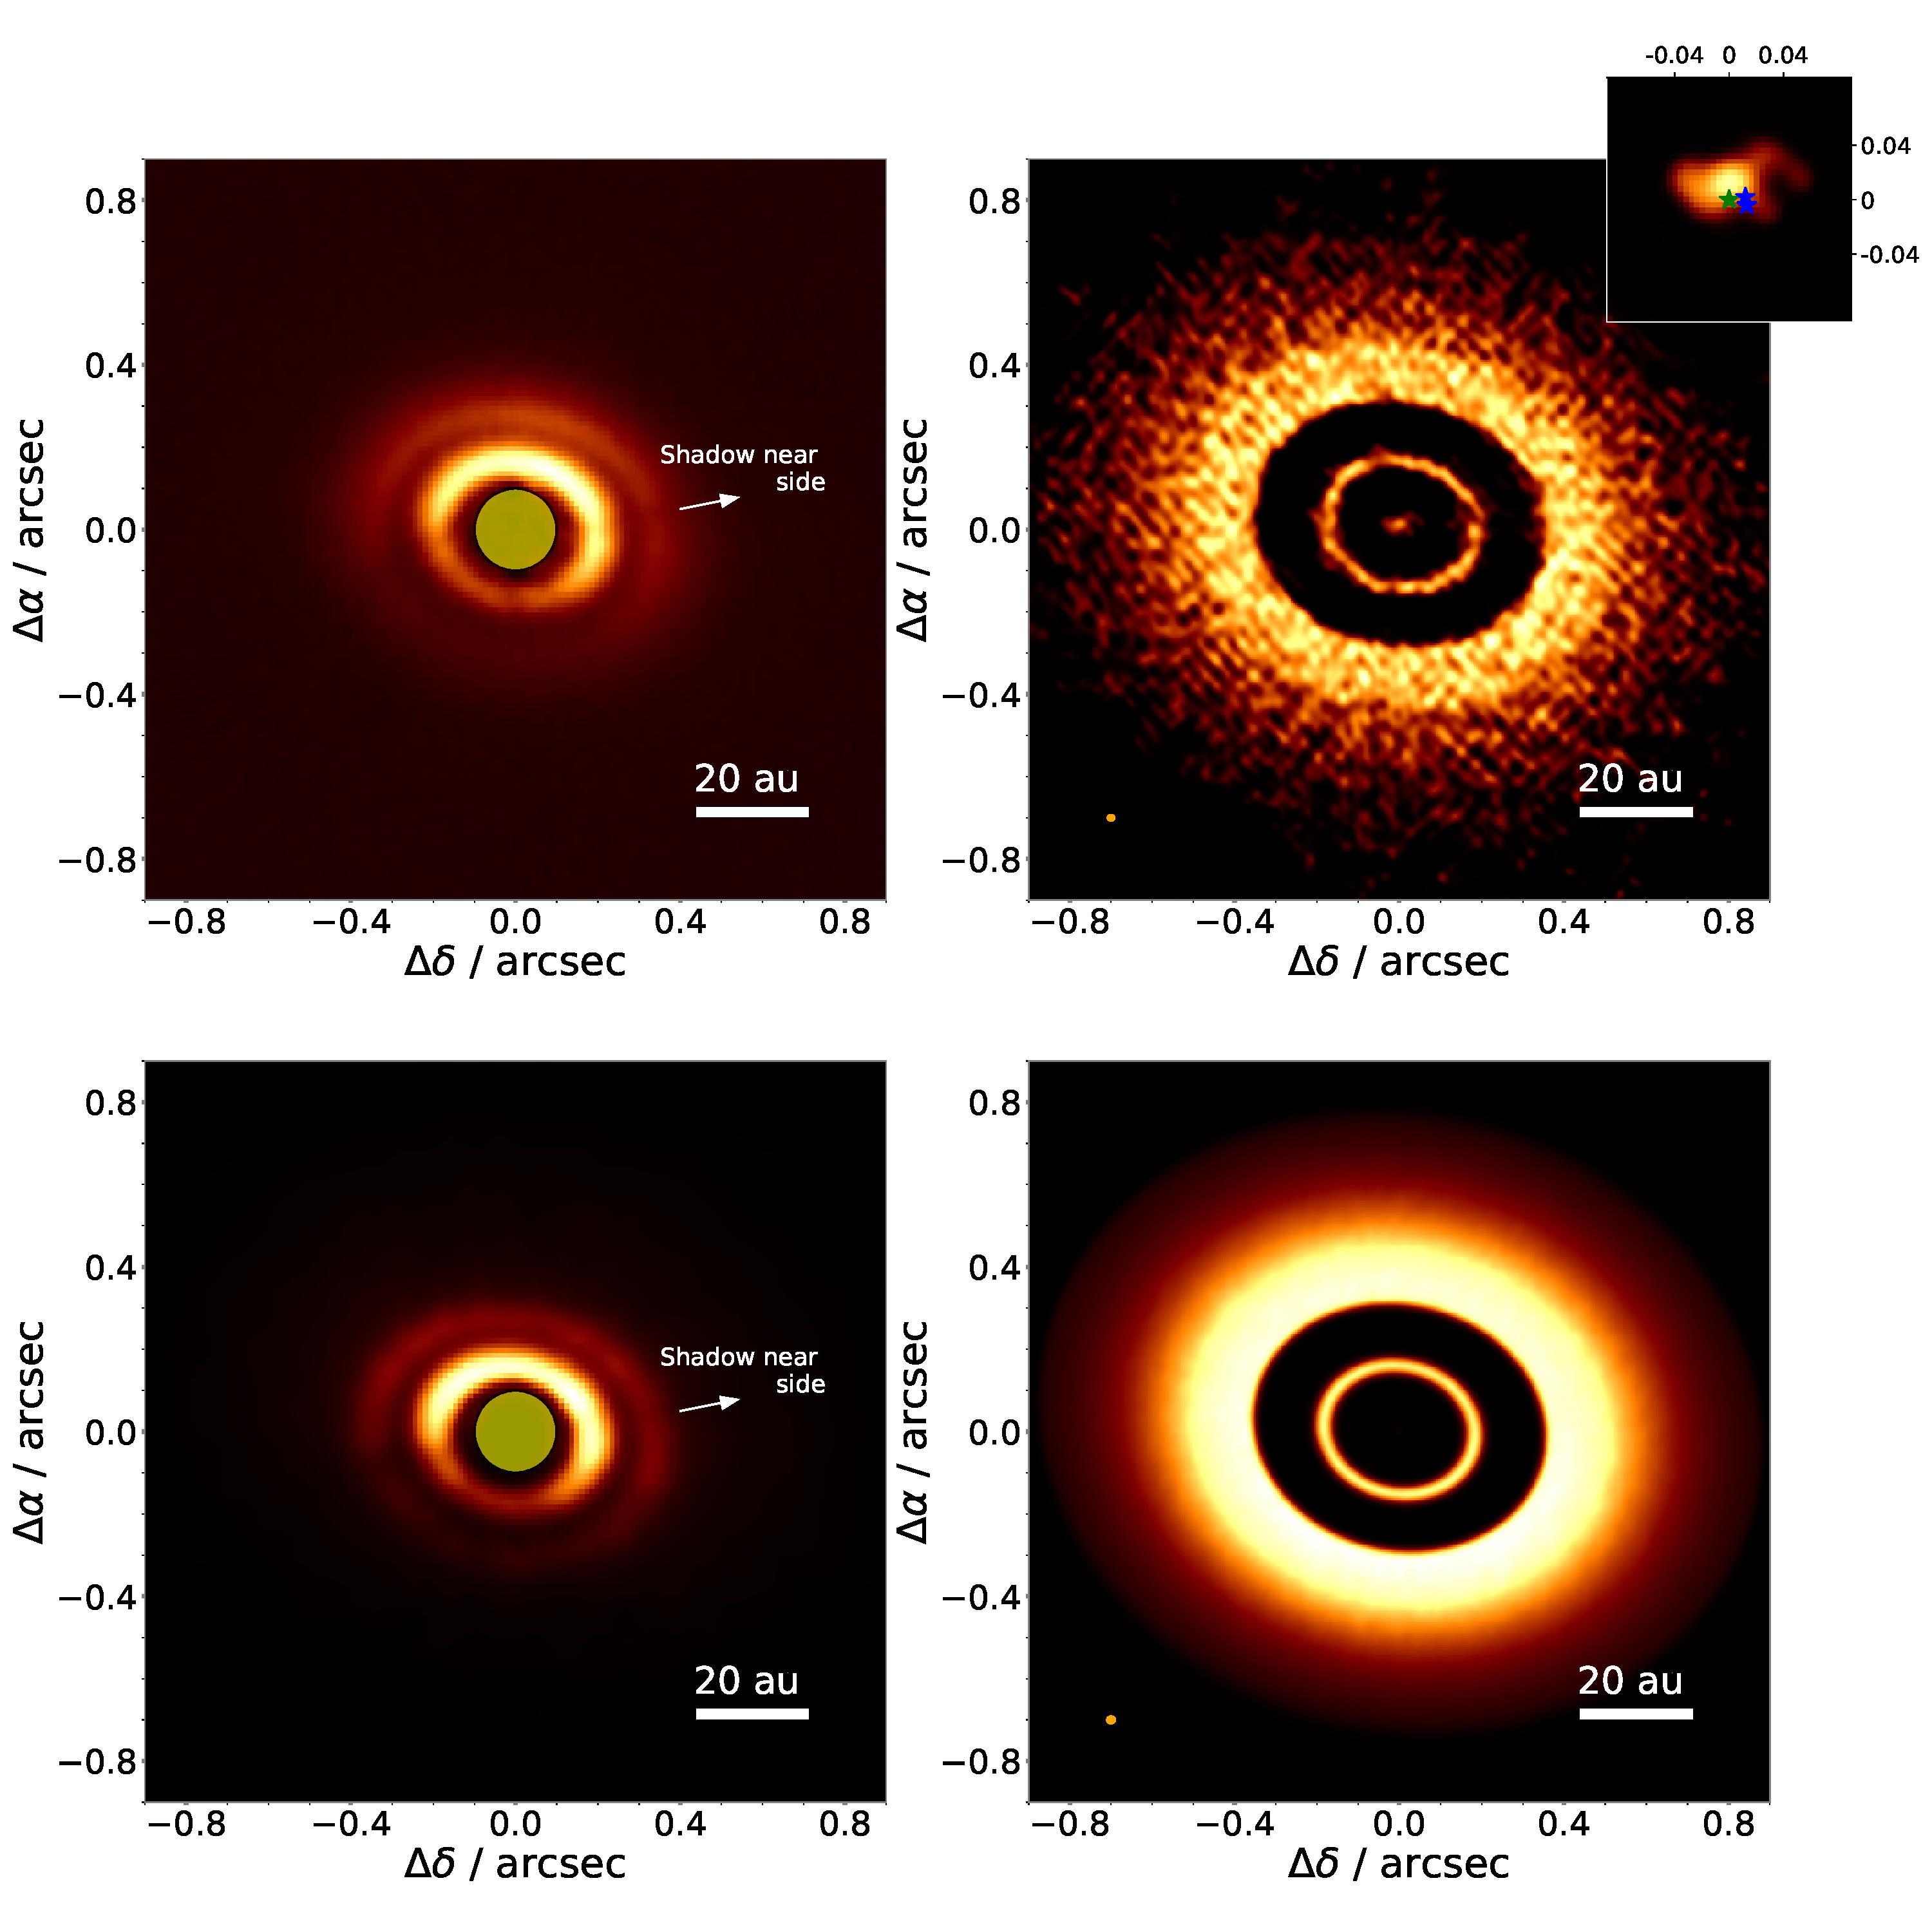
\includegraphics[width=\textwidth]{hot_two_E.pdf}
  \caption{Comparison of observations \phil{(top)} and simulated images \phil{(bottom)} at 1.65\,$\micron$ \phil{(left)} and 1.3 mm continuum \phil{(right)} of the circumbinary disc orbiting V4046\,Sgr. \st{From top to bottom: DPI image and ALMA Band 6 observations; simulated images of the parametric model.} \phil{\textit{Top left panel:}} SPHERE-IRDIS \textit{H}-band image with a yellow filled circle that represents the N\_ALC\_YJH\_S coronagraph with a radius of $\sim0\farcs12$, or $\sim$8.6\,au at 72.4\,pc. \phil{\textit{Top right panel:}} 1.3\,mm continuum {\tt uvmem} model image. The yellow ellipse shows the size of the natural-weighted beam ($ 0\farcs062 \, \times \, 0\farcs055$), and the small orange ellipse shows an estimated {\tt uvmem} beam size ($\sim0\farcs035 \, \times \, \sim0\farcs031$). The inset zooms into the central emission, and the green star marks the \st{star positions} \phil{binary position}. \phil{\textit{Bottom left panel:}} synthetic image at 1.65\,$\upmu$\phil{m}. \phil{\textit{Bottom right panel:}} synthetic image at 1.3\,mm. . For all the images in the figure the colour scale is linear.}
  \label{fig:images_vs_simulated}
\end{figure*}

Ring13 is surprisingly narrow and seems to be off-centred relative to the GAIA stellar position, at the origin of coordinates in Fig.~\ref{fig:images_vs_simulated}. We determined the ring's centre and orientation by minimising the dispersion of the disc radial profiles from 6\,au to 19\,au, by using the {\tt MPolarMaps} package described in Casassus et al. (2021, in prep). The resulting disc orientation is set at a position angle  (PA) of 77.31$\pm$0.03\,$\degr$, with an  inclination of 32.96$\pm$0.02\,$\degr$, and the optimal ring  centre is at $\Delta \alpha = -4\pm0.02$\,mas $\Delta \delta = 13\pm0.05$\,mas relative to the GAIA position of the stars. The offset of the center of the cavity and the nominal stellar positions is entirely consistent with a pointing error, since the pointing accuracy of ALMA is usually taken to be 1/10 of the natural-weights beam, at 1\,$\sigma$, or $\sim$6\,mas in this case. ***ANTONIO PLEASE CONFIRM AND PROVIDE A REFERENCE ****

The ring width can be measured in polar coordinates by fitting 1-D Gaussians, thus obtaining a width and centroid at each azimuth. On average, we obtained a FWHM of 2.87$\pm$0.50\,au, and a stellocentric radius of 13.32$\pm$0.26\,au (See Fig.~\ref{fig:polarring}). As the {\tt uvmem} model image has an effective angular resolution of $\sim$1/3 that of the natural-weighted beam ($0\farcs062 \,\times \, 0\farcs055$), we see that Ring13 is marginally resolved. After subtraction of the approximate {\tt uvmem} resolution ($\sim0\farcs035 \, \times \, \sim0\farcs031$), the ring width is $\sim$1.50$\pm$0.72\,au.

In a second optimization of the disc orientation, but this time aiming for Ring24 with a radial domain from 20\,au to 70\,au, we obtained a PA of 76.86$\pm$0.02\,$\degr$, with an inclination of 33.92$\pm$0.01\,$\degr$ and a centre at $\Delta \alpha = 2\pm0.02$\,mas $\Delta \delta = 12\pm0.02$\,mas relative to the stars. We see that both Ring13 and Ring24 both share a very similar orientation and centre, given the errors. However, perhaps due to the joint effect of all these small differences, we can see that there are some hints for a somewhat different orientation, as summarised in Fig.~\ref{fig:polarring}.

Interestingly, the ALMA image also detects faint 1.3\,mm continuum emission near the stellar positions (See the inset in Fig.~\ref{fig:images_vs_simulated}). Since this faint central emission is larger than the angular resolution, it is probably stemming from thermal emission from  large dust grains rather directly from the stars. The main blob of this dust structure is at a estimate distance of only $0\farcs012\pm0\farcs002$, or $\sim$0.9\,au from the binary system, and may be part of \phil{an} inner disc introduced in the RT model to match the SED (see Sec.~\ref{sec:model} below). 

%match the small grain ring called Ring6 introduced in the RT model to match the SED (see Sec.\,\ref{sec:model} below). If so, then given that the binary phase at the time of the observations is PA=347\,$\degr$, so that the secondary lies roughly northwards of the primary, it may be that the northern side of Ring6 is shadowed, resulting in a seemingly lopsided geometry.

The scattered-light image \st{shown} in \phil{the top left panel of} Fig.~\ref{fig:images_vs_simulated} also shows a double ring structure in the micron-sized dust distribution. The observed morphology presents an inner cavity of $\sim$10\,au in radius and two rings located at 14.10$\pm$0.01, coincident with Ring13, and 24.62$\pm$0.08\,au, coincident with Ring24, with a small gap between them at $\sim$20\,au. The observed second ring matches the inner wall of the 1.3\,mm continuum emission outer ring \citep{Ru_z_Rodr_guez_2019}. Two other important features that are present in the image are: the brightness asymmetry and the shadows projected on the disc produced by the close binary system as they eclipse each other, discovered by \citet{dOrazi}.

The binary phase reported by \citet{dOrazi} in the scattered-light observation is at a position angle (PA) of 265\,$\degr$, east of north. Using this measurement, the binary phase was calculated at the time of the ALMA observation at a PA of $\sim$80\,$\degr$. There is no hint of radio decrements in either Rings13 nor in Ring24 that would match shadowing at this PA. This could be explained by inefficient disc cooling compared to the speed of the illumination pattern \citep[see ][ for estimates of this cooling timescale]{Casassus2019MNRAS.486L..58C}. 

\begin{figure}
    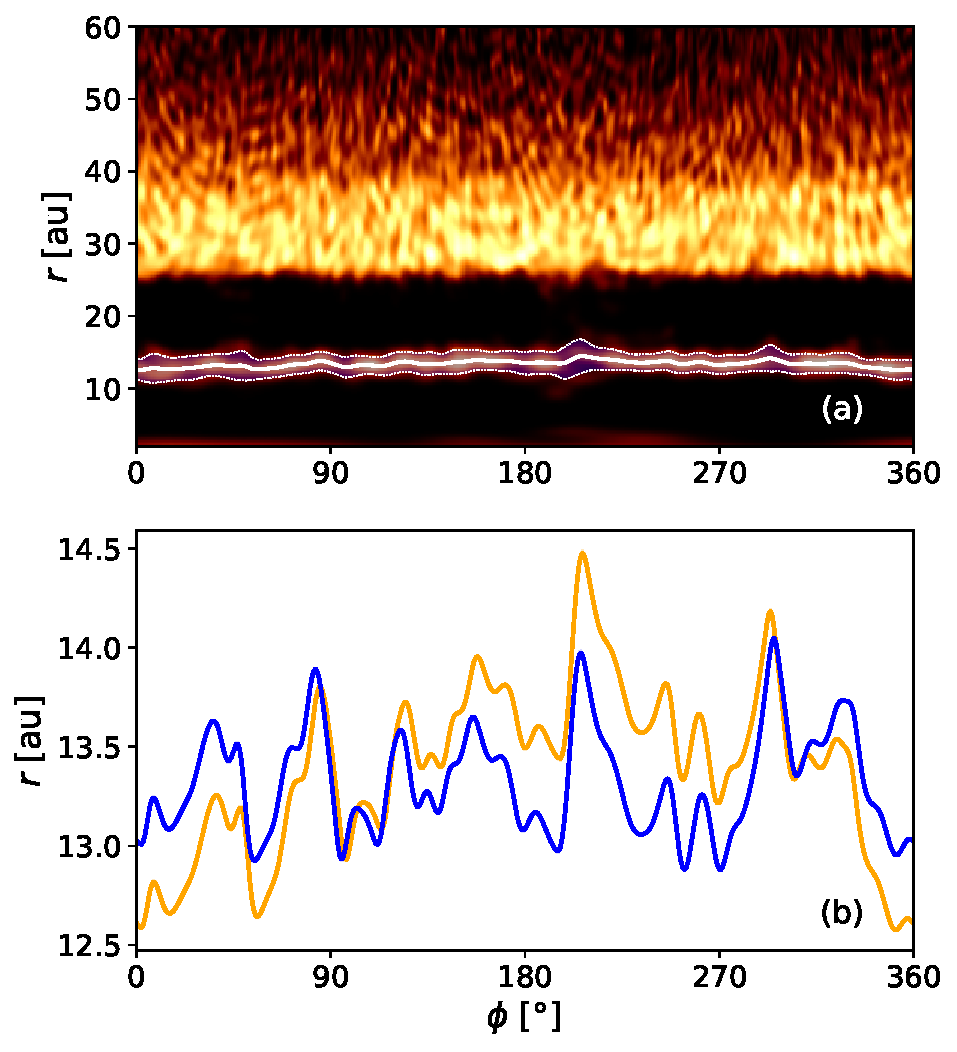
\includegraphics[width=\columnwidth]{polar_ring_aprox_and_diff_inner.pdf}
    \caption{(a) Polar decomposition of the 1.3\,mm continuum image, using the orientation of Ring24. We trace Ring13 using the centroids (solid line) and width of radial Gaussian fits (blue region between the dotted lines). (b) Centroid of Ring13, for two disc orientations: the orange line corresponds to the same trace as in a), while the blue line is obtained for the inner ring orientation.}
    \label{fig:polarring}
\end{figure}

The observed SED was collected from data in the literature \citep{1988iras....7.....H, 1990A&A...234..230H, Jensen_97, 2000A&A...355L..27H, 2001KFNT...17..409K, 2003yCat.2246....0C, 2007PASJ...59S.369M, 2008PASP..120.1128O, 2010A&A...514A...1I, 2012yCat.2311....0C}, available online in \textsc{vizier}. We also  used  archival \textit{Spitzer} IRS spectroscopic data (see Fig.~\ref{fig:SED}). 

\begin{figure}
	\centering
	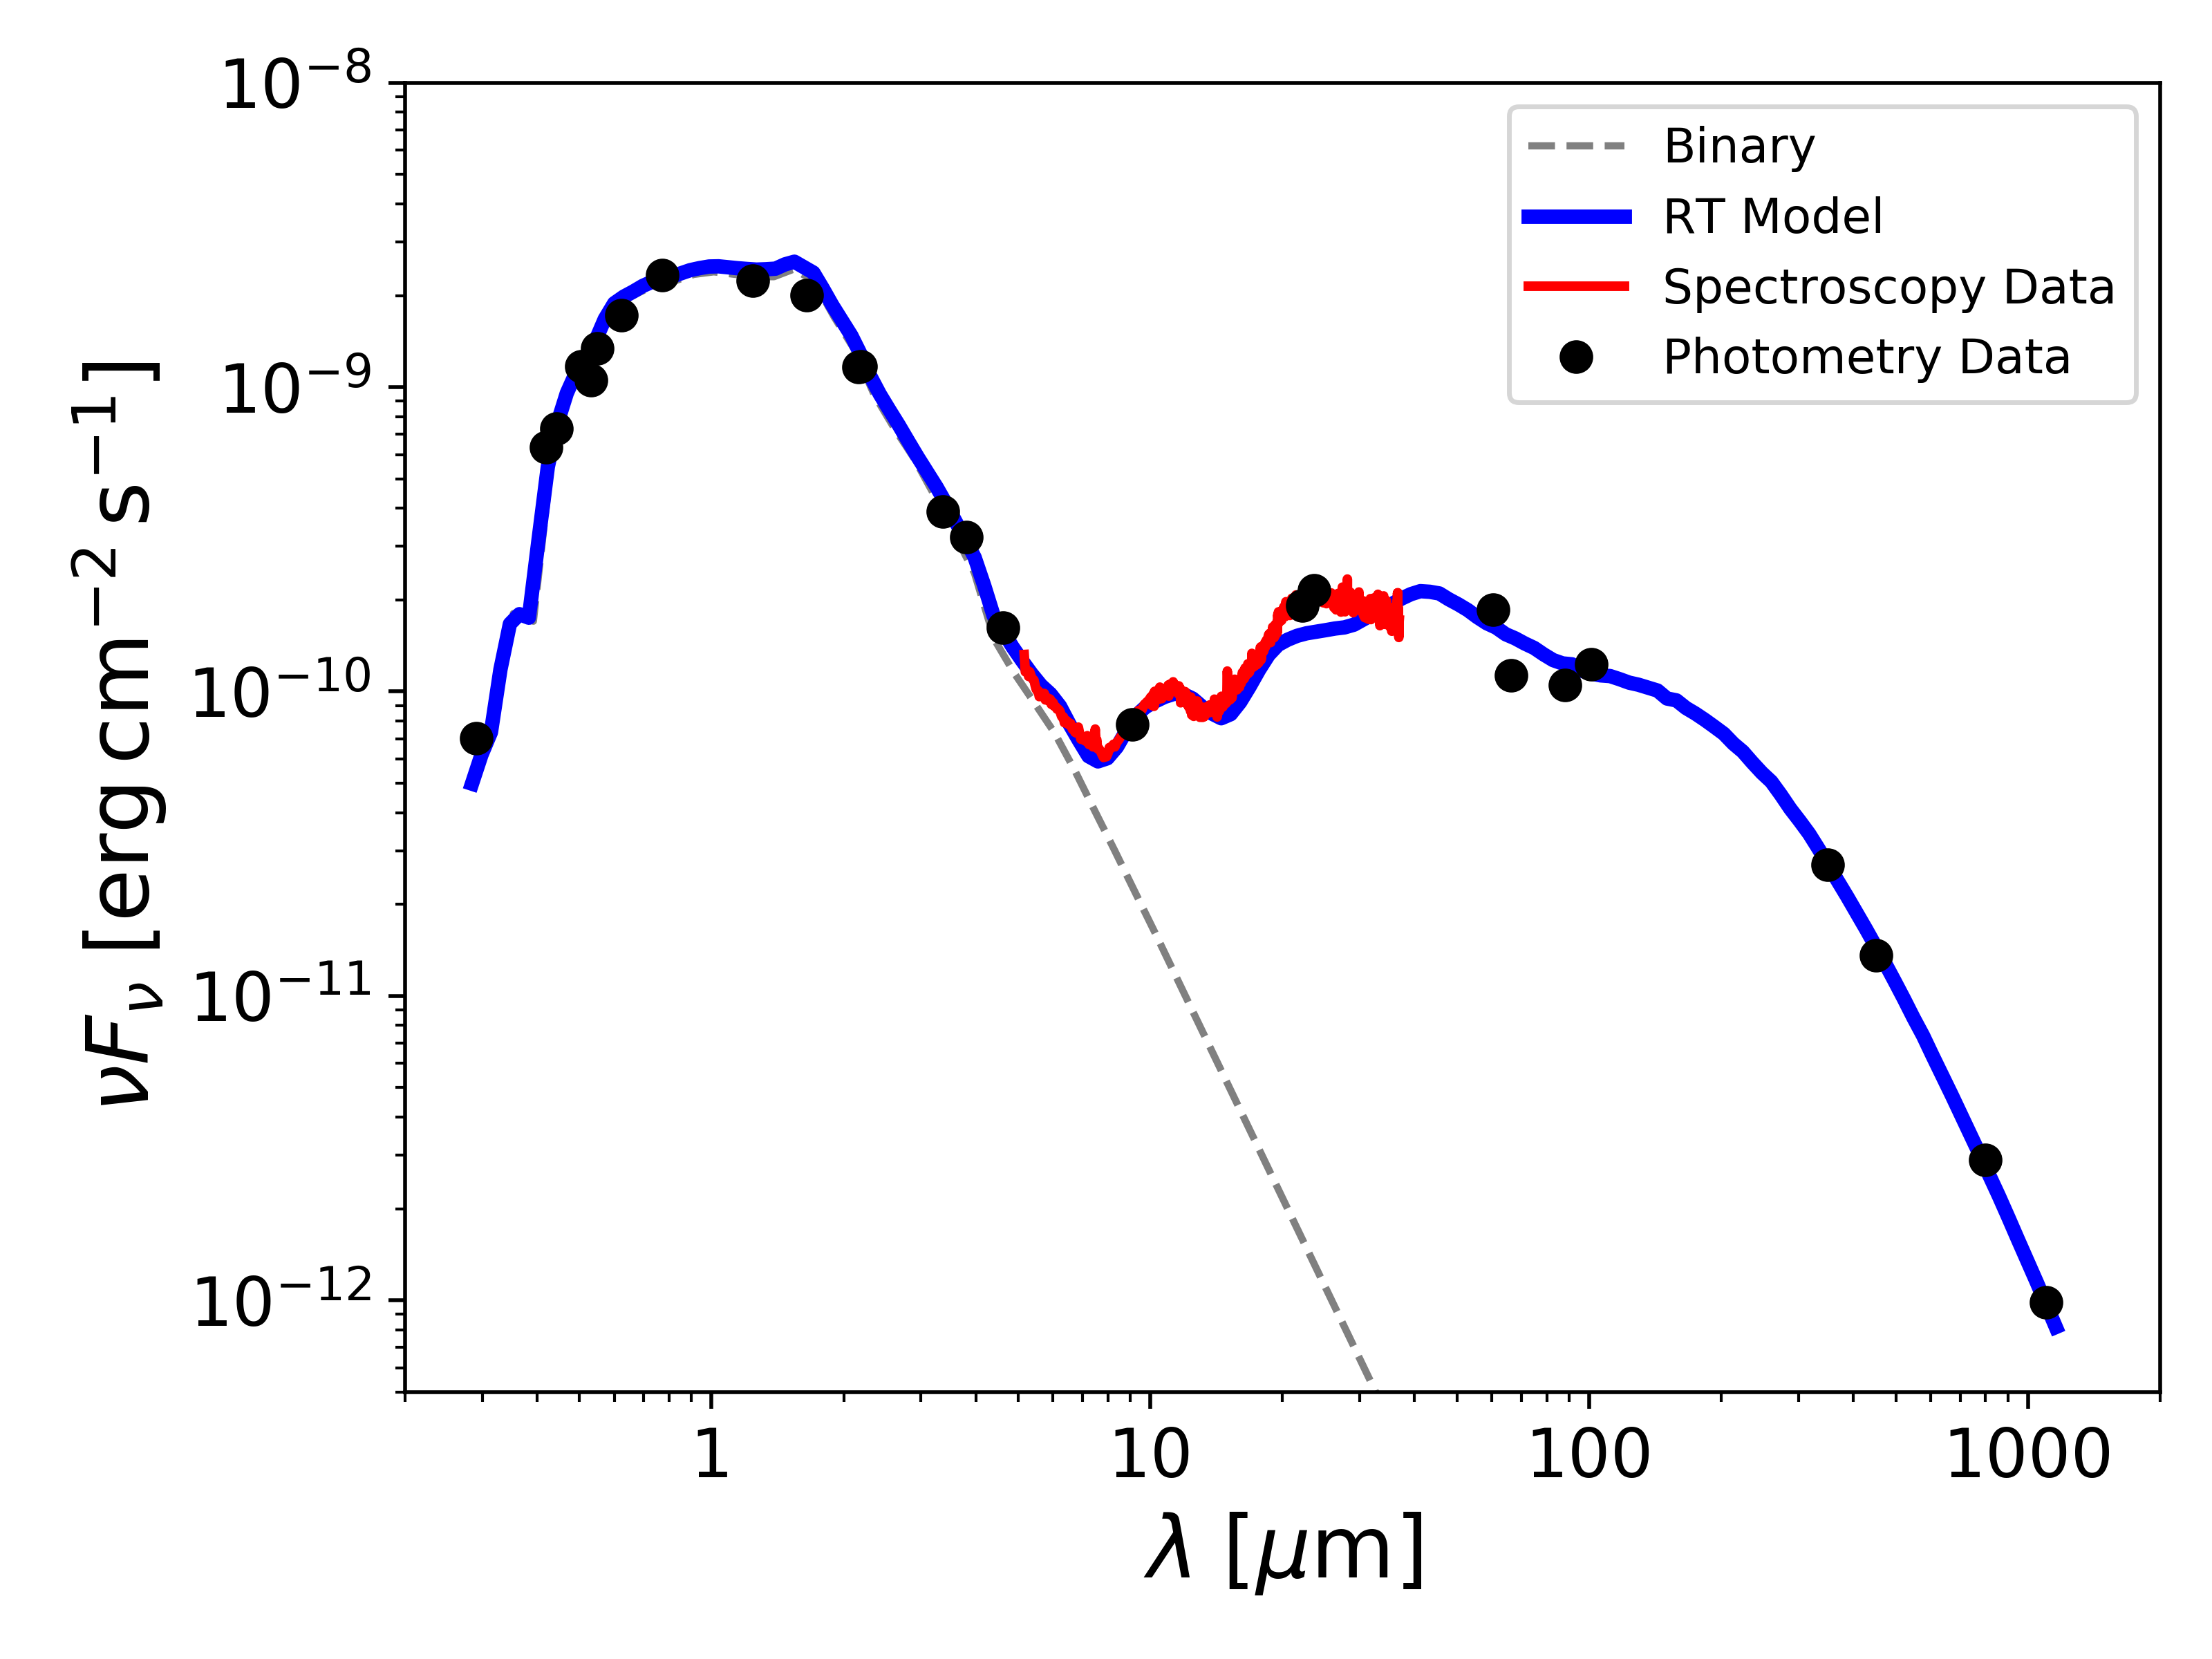
\includegraphics[width=\columnwidth]{SED_.png}
    \caption{\phil{Change labels in legend: binary instead of stars, RT Model} \phil{Spectroscopy Data, Photometry Data.} The observed SED of V4046\,Sgr (black points and solid red curve) compared with the model (blue). The black points represent the measured photometry and the red line shows an archival \textit{Spitzer} IRS spectrum. The dashed silver curve shows the emission of the stellar photosphere model.}
    \label{fig:SED}
\end{figure}

\section{Parametric radiative transfer model} \label{sec:model}

The multi-frequency data can be interpreted in terms of a physical structure using radiative transfer predictions, for which we used the \textsc{radmc3d} package \citep{Dullemond_2012}. The general framework of the parametric model that we used is similar to that in \citet{2018MNRAS.477.5104C} for DoAr\,44, and the initial model values were inspired from those in \citet{Rosenfeld_2013}. Through trial and error, we found a set of values for the parameters that correctly fit the available data. The final structure of the parametric model is summarised in  Fig.~\ref{fig:profiles}.

The stars were modeled using two Kurucz photospheres models \citep{1979ApJS...40....1K, 1997A&A...318..841C}, with T$_{\mathrm{eff},1} =$ 4350\,K, R$_{*,1} =$ 1.064\,R$_{\sun}$, M$_{*,1} =$ 0.90\,M$_{\sun}$ and T$_{\mathrm{eff},2} =$ 4060\,K, R$_{*,2} =$ 1.033\,R$_{\sun}$, M$_{*,2} =$ 0.85\,M$_{\sun}$ respectively and with an accretion rate of \st{$\mathrm{log}(\,\dot{\mathrm{M}/(\mathrm{M}_{\sun}\,\mathrm{yr^{-1}})}) = -$9.3} \phil{[replace by:]} $\mathrm{log}(\,\dot{\mathrm{M}}/(\mathrm{M}_{\sun}\,\mathrm{yr^{-1}})) = -$9.3 for both cases to include excess UV due to stellar accretion \citep{10.1111/j.1365-2966.2011.19366.x}. The stars were placed at a mutual separation of 0.041\,au, so that their centre of mass coincides with the origin, and oriented at a PA of 250\,$\degr$, so that the secondary lies to the NWW from the primary, thus casting the same shadow as observed by \citet{dOrazi}.

Reproducing the radial and vertical structure of the V4046\,Sgr disc turned out to be challenging. We built the model in terms of the gas distribution, and with two different dust populations: larger grains that are vertically settled and dominate the total dust mass, and a population of smaller grains that are uniformly mixed with the gas and reach \phil{higher regions} \st{larger heights} above the mid-plane. 

Assuming a three dimensional model in a cylindrical reference frame with coordinates ($r$, $\theta$, $z$) \phil{[just for conventional reasons, I would use $\phi$ instead of $\theta$]}, the gas density ($\rho_{\mathrm{gas}}$) distribution follows
\begin{equation}
  \rho_{\mathrm{gas}}(r,z) =\frac{\Sigma_{\mathrm{gas}}(r)}{\sqrt{2\pi} \, H(r)} \mathrm{exp}\left[-\frac{1}{2} \left(\frac{z}{H(r)}\right)^2\right],
\end{equation}
where $H(r)$ is the scale height profile and $\Sigma_{\mathrm{gas}}(r)$ is the gas surface density profile. 

The parametric scale height profiles for the gas and for each dust population are 
\begin{equation}
    \label{scale}
  H(r)=\chi \, H_{\circ} \, [r/r_{\circ}]^{\psi(r)},
\end{equation}
where $H_\circ$ is the scale height at \st{r} \phil{$r$}= $r_\circ$, $\psi$ is the flaring index and $\chi$ is a scaling factor (in the range $0-1$) that mimics dust settling. The gas and the small dust \phil{(sd)} grains have no settling, so \st{$\chi_{gas}$} \phil{$\chi_{\rm gas}$ = $\chi_{\rm sd}$} = 1. The radial spread of Ring13 appears about five times wider in the gas-tracing NIR observations than in the fluxes received from larger grains with ALMA. We assume that the same ratio holds in the vertical direction (due to the settling of larger grains towards the disk's midplane), leading to \st{$\chi_{ld}=1/5$} \phil{$\chi_{\rm ld}=0.2$ [adapt this in case you changed the model to 0.3]}.

For the \st{vertical structure} \phil{scattering surfaces}, \citet{dOrazi} found flaring angles of $\varphi$ = 6.2$\pm$0.6\,$\degr$ for the inner ring and $\varphi$ = 8.5$\pm$1.0\,$\degr$ for the outer one. Our model uses the same values, with two different flaring \st{indexes} \phil{indices, $\psi_1$ and $\psi_2$} \st{$\psi$}. The separation between the two values were set at $r$ = 18\,au with \phil{$\psi_1=0.15$} for Ring6 and Ring13, and \phil{$\psi_2=0.5$} for Ring24. The scale height is $H_\circ = 0.45$\,au at $r_\circ = 18$\,au.

We propose a three ringed structure \phil{to reproduce the observations.} \phil{We separate the disk into four individual regions:}\st{, so we defined the total gas surface density by a combination of four individual components:} the inner disc, Ring6, Ring13 and Ring24. The \st{total} \phil{combined} gas surface density \phil{profile} is then  given  by:
\begin{equation}
  \Sigma_{\mathrm{gas}}(r) = \Sigma_{\mathrm{inner\,disc}} + \Sigma_{\mathrm{Ring6}} + \Sigma_{\mathrm{Ring13}} + \Sigma_{\mathrm{Ring24}}
\end{equation}

The inner disc follows a power law function defined by
\begin{equation}
  \Sigma_{\mathrm{inner\,disc}}(r) =\Sigma_\mathrm{c} \left(\frac{r}{R_\mathrm{c}}\right)^{-\gamma}  \, \mathrm{exp}\left[-\left(\frac{r}{R_\mathrm{c}}\right)^{2-\gamma}\right],
\end{equation}
where $R_c$ is a characteristic radius and $\gamma$ is the surface density \st{gradient} \phil{power-law index}. We used $R_c$ = 16\,au, $\Sigma_\mathrm{c} =2.7\times10^{-4}$\phil{\,$\mathrm{g\,cm^{-3}}$} and a fixed $\gamma$ = 1 as it is a typical value for discs \citep{Andrews_2009,Andrews_2010}. \st{The gas surface density begin at 0.3\,au, out of the zone expected to be cleared by dynamical interactions with the central binary} \citep{Art_Lu}, \st{which is expected to be $\sim$0.2\,au.} \phil{Our model extends from 0.3\,au outwards, as the interior is expected to be} \phil{cleared by dynamical effects of the central binary} \citep{Art_Lu}. 

We \st{chose} \phil{choose} to use Gaussian profiles to parameterize Ring6 and Ring13,
\begin{equation}
  \Sigma_{\mathrm{Ring}}(r) = \frac{\Sigma_\circ}{\sqrt{2 \pi} \sigma}
  \, \mathrm{exp}\left[-\frac{1}{2}\left(\frac{r-\mu}{\sigma}\right)^{2}\right],
\end{equation}
where we define constants that correspond to the centroid radii \{$\mu_{\mathrm{Ring6}}=5.5$\,au, $\mu_{\mathrm{Ring13}}=15$\,au\}, ring widths \{$\sigma_{\mathrm{Ring6}}=1$\,au, $\sigma_{\mathrm{Ring13}}=2.05$\,au\}, and normalizations \phil{[this $\Sigma$ cant be right? Also, units for density!]} \{ $\Sigma_{\circ,\mathrm{Ring6}}=8\times10^{12}$, $\Sigma_{\circ,\mathrm{Ring13}}=4.2\times10^{13}$\} for both components separately.

For Ring24 we used the same power law \st{than} \phil{as for} the inner disc but scaled by \st{a $\delta_{\mathrm{sd}}$ factor} \phil{an empirically obtained factor, $\delta_{\mathrm{sd}}$= 5.3$\times 10^4$}:
\begin{equation}
  \Sigma_{\mathrm{Ring24}} = \Sigma_{\mathrm{inner\,disc}}(r)\, \delta_{\mathrm{sd}},
\end{equation}
\st{with $\delta_{\mathrm{sd}}$ = 5.3$\times 10^4$.} \st{But the inner wall} \phil{The inner edge} of Ring24 follows a different \st{behaviour} \phil{profile}. Between $R_\mathrm{in}$ and $R_\mathrm{peak}$, which respectively mark  the \st{beginning} \phil{inner edge} and the \phil{location of} maximum density \st{peak} of the outer ring, the gas density profile is multiplied by an additional factor
\begin{equation}
    \epsilon(r) = \left(\frac{ r - R_\mathrm{in}}{R_\mathrm{peak} - R_\mathrm{in}}\right)^3.
\end{equation}
This parameter \st{allow} \phil{allows} us to model a smoother inner \st{wall} \phil{edge} of the outer ring, with $R_\mathrm{in,gas}$ = \st{18.\,au} \phil{18.0\,au} and $R_\mathrm{peak,gas}$ = 26.8\,au. This factor is also applied to the large dust population with $R_\mathrm{in,ld}$ = 24.7\,au and $R_\mathrm{peak,ld} = R_\mathrm{peak,gas}$. 

The total dust-to-gas mass ratio is taken to be $\zeta = 0.047$ \citep[as in][]{Rosenfeld_2013}. The small dust grains are assumed to only make up for a fraction of $f_\mathrm{sd}=1\%$ of the total dust mass. As small dust is typically tightly coupled to the gas dynamics, its density profile is expected to follow the gas density. Then the density of small dust can be calculated as:
\begin{equation}
\rho_{\mathrm{small-dust}}(r,z)=\rho_{\mathrm{gas}}(r,z)\, f_{\mathrm{sd}} \: \zeta .
\end{equation}

Since the large dust grains are less coupled to the gas, their distribution has some important differences that require a special parameterisation, with a large inner cavity, a larger gap between the rings and a break in the outer ring. We also truncated the \st{model large-grain density} \phil{profile of large dust grains} at 64\,au. \st{The large-dust surface density profile is} \phil{It is then} defined by the sum of its two components
\begin{equation}
  \Sigma_{\mathrm{ld}}(r) = 
  \Sigma_{\mathrm{Ring13,ld}} + \Sigma_{\mathrm{Ring24,ld}}.
\end{equation}

For the inner ring, we \st{chose} \phil{choose} a Gaussian profile parameterized with centroid radius $\mu_{\mathrm{Ring13, ld}}=13.38$\,au, ring width of $\sigma_{\mathrm{Ring13,ld}}=0.54$\,au and $\Sigma_{\circ,\mathrm{Ring13,ld}}=3\times10^{13}$. For Ring24 we used the same profile \st{of} \phil{as for} the gas, but with the difference that, in an effort to recreate the break seen in the outer ring, we \st{chose} \phil{choose} different values for \st{$\gamma$ = -5} \phil{$\gamma = -5$} and $R_c$ = 38\,au between 28.6 and 35.6\,au. The surface density \st{of the outer ring of large grains dust} \phil{for large dust grains in the outer ring} is thus given by
\begin{equation}
    \Sigma_{\mathrm{Ring24,ld}} = \Sigma_{\mathrm{c}} \left(\frac{r}{R_{\mathrm{c}}}\right)^{-\gamma} \exp\left[-\left(\frac{r}{R_{\mathrm{c}}}\right)^{2-\gamma}\right]\,\delta_{\mathrm{ld}}(r),
\end{equation}
where
\begin{equation}
  \delta_{\mathrm{ld}}(r) =
  \begin{cases}
  0                 & r < 24.6\text{\,au} \\
  6.24 \times10^{4} & 24.6 < r < 28.6\text{\,au} \\
  2.78 \times10^{4} & 28.6 < r < 37\text{\,au} \\
  2 .14 \times10^{5} & 37   < r < 64\text{\,au.} \\
  \end{cases}
\end{equation}
Then the final density of large dust can be calculated as
\begin{equation}
\rho_{\mathrm{large-dust}}(r,z)=
\frac{\Sigma_{\mathrm{ld}}(r)}{\sqrt{2\pi} \, H(r)} \mathrm{exp}\left[-\frac{1}{2} \left(\frac{z}{H(r)}\right)^2\right] \, f_{\mathrm{ld}} \: \zeta .
\end{equation}

The two different populations of dust grains correspond to small grains, with radii ranging from 0.4\phil{\,$\micron$} to 1.5\,$\micron$, and large dust grains, with radii from 0.4\,$\micron$ to 10\,mm. We computed the dust opacities using the {\tt bhmie} code provided in the \textsc{radmc3d} package, with a mix composed of 60\% silicate, 20\% graphite and 20\% ice. 

The observed near-far asymmetry in the DPI image is suggestive of a strongly forward-scattering phase function. In order to reproduce a similar asymmetry, we used much larger grains than typically used in the RT modelling of such near-IR data \citep[e.g.,][]{2018MNRAS.477.5104C}. 

The simulated DPI image at 1.65\,$\micron$ in Fig.~\ref{fig:images_vs_simulated} was obtained with the scattering matrix calculated by the {\tt makeopac.py} script provided in the \textsc{radmc3d} package. As a way of reproducing the \textit{H}-band image, we used a different grain size distribution, where we \st{used} \phil{centred} a Gaussian \st{distribution} \st{centred} at 0.4\,$\micron$ \st{but} \phil{,}  smeared out by 30\%, and \phil{distributed over 20 bins within that range} \st{with 20 grain size bins within that range}. This distribution applies only to generate the NIR $Q_\phi$ image. To produce this $Q_\phi$ image we performed a linear combination of the two orthogonal linear polarizations \textit{U} and \textit{Q}, following \citet{Avenhaus_2017}, which gives a representation of an unbiased estimate of the polarized intensity image.

\begin{figure}
	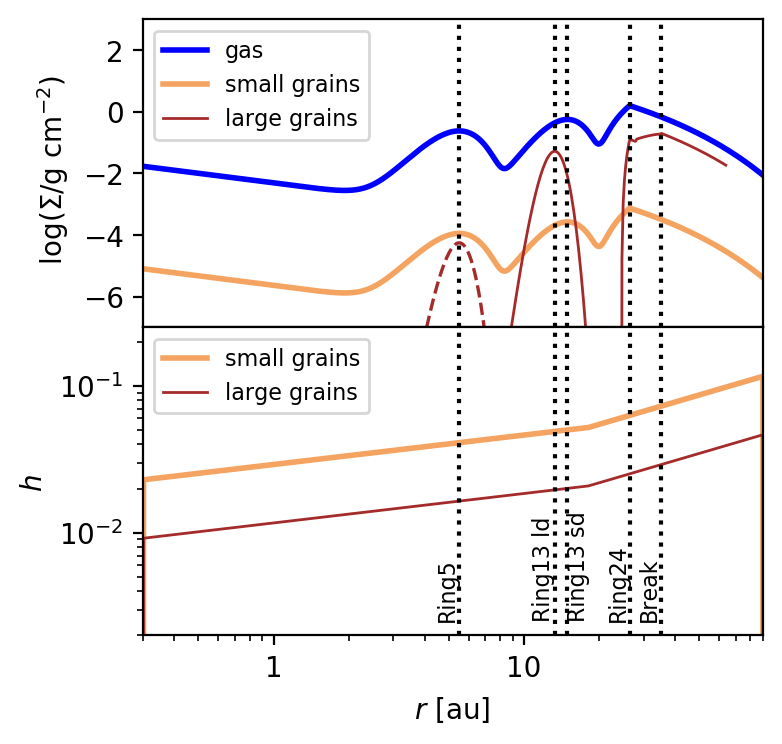
\includegraphics[width=\columnwidth]{allprofiles.png}
        \caption{{\bf Top:} surface density profiles for \st{the} gas, \st{the}large and small \phil{dust grains} \st{grain populations}. {\bf Bottom:} Aspect ratio profile $h(r)= H(r)/r$. The \st{dashed} \phil{dotted} lines crossing both panels correspond to transition radii in the parametric model.}
    \label{fig:profiles}
\end{figure}

The inner radius of the model grid was set to 0.1\,au,  and the outer radius \st{of} \phil{to} 100\,au, which is large enough for the dust disc to \st{become} \phil{be} undetectable. We set the values of the inclination \st{an} \phil{and} disc position angle \phil{to} \st{as} the same as \st{those} obtained from the ALMA observation in Section~\ref{sec:Observations}, \st{so} \phil{such that} the model has an inclination of i = 32.96\,$\degr$ and a P.A. = 77.31\,$\degr$. Finally, the distance is set \st{at} \phil{to} d = 72.4\,pc \citep{Gaia}.

\section{Model results and discussion} \label{sec:results}

While certainly not unique, our parametric model is fairly successful in reproducing the available data. The simulated images and the SED of the model are shown in Fig.~\ref{fig:images_vs_simulated} and Fig.~\ref{fig:SED} respectively.

The simulated image at 1.65\,$\micron$ shows a similar radial structure to the one visible in the observations, displaying a two ringed disc, where Ring6 hides under the artificial coronagraph. The visible asymmetry in the SPHERE observations is reproduced using \st{relative} \phil{relatively} large grains, $\sim$0.4\,$\micron$, as smaller grains did not result in such strong forward scattering. As \citet{refId0} \phil{[This citation looks strange, the T. should not be there]} \st{states} \phil{state}, this forward scattering peak \st{that is} present in the observation may indicate that the dust grains in the disk surface are \phil{relatively} large, suggesting that the disc is depleted of very-small grains. Interestingly, the model accurately shows the shadows described by \citet{dOrazi} that are present in the SPHERE-IRDIS image.  

\begin{figure}
	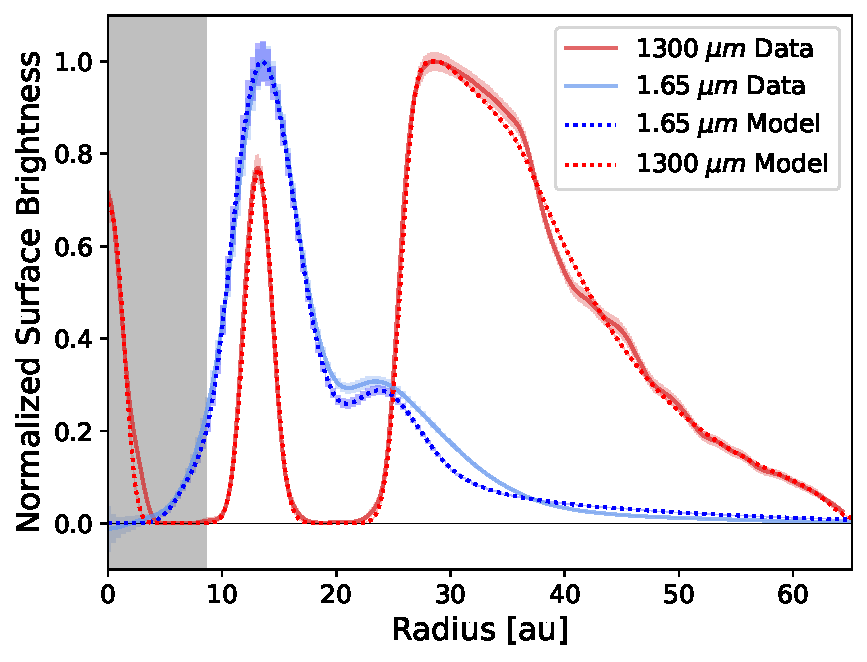
\includegraphics[width=\columnwidth]{comp_fig_all_profiles_au.pdf}
    \caption{Comparison of the surface brightness profiles extracted from the deprojected synthetic images and observed \textit{H}-band and 1.3\,mm continuum images. The grey shaded area represents the radius of the artificial coronagraph used in the simulations (i.e., $\sim0\farcs 12$, or $\sim$8.6\,au at 72.4\,pc).}
    \label{fig:radprofiles}
\end{figure}

The simulated 1.3\,mm continuum image reproduces the two observed rings: the faint Ring13 and the brighter Ring24. As the radial profiles obtained from the simulated images of the model closely resemble those deduced from the observations (Fig.~\ref{fig:radprofiles}), we can assume that the model provides a possible approximation of the disc structure, including the dimensions of Ring13. Accordingly, taking the parametric model values for Ring13 \st{we have that} \phil{,} it has a radius of 13.36\,au, a FWHM of 1.30\,au, and a scale height FWHM of the millimetre-size dust of 0.65\,au. The total dust mass of Ring13 is about 1.1\,M$_{\earth}$ in the model. In turn, \st{in} our model \phil{reproduces the observations of} Ring24 \st{reaches} \phil{with} peak intensity at $\sim$30\,au, \st{then breaks} \phil{and break} at $\sim$36\,au\st{, as in the observations, and has}\phil{. It contains} a total dust mass of $\sim$50\,M$_{\earth}$. The model predictions for the millimetre-size dust population in Ring13 are close to the measurements, with only a 0.06\,au difference in the centroid location of the ring, and a 0.2\,au difference in the width estimation. Using the large \st{grains} \phil{grains'} scale height \phil{at Ring13} of 0.31\,au \st{at Ring13}, and a measured width of 1.50\,au, the ring is $\sim$4.8 times more extended  radially than vertically.

The observed structure may point to the existence of planet-disc interactions within this system, where a giant planet depletes its orbit of gas and dust material. A possible  constellation in this scenario is therefore the presence of two giant planets in the disc, one planet between the star and Ring13, and one planet between Ring13 and Ring24. As \citet{Ru_z_Rodr_guez_2019} suggest, the putative planet between Ring13 and Ring24 may be a giant planet with a mass within the range of 0.3$-$1.5\,$\mathrm{M}_{\mathrm{Jup}}$. This idea is supported by the similarity to the structure around HD\,169142 which \citet{2020arXiv200711565B} reproduced by including several giant planets. 


The effective beam size of the presented ALMA observations marginally resolves the width of Ring13 to be $w_\mathrm{d} = 1.50\mathrm{au}$. %The most suitable RT model demands a density distribution of small grains and gas that is radially more extended, with an approximate width of $7.5\mathrm{au}$. Although the RT model ascribed step functions to gas and dust densities, in a more physical scenario the density should roughly follow a Gaussian distribution.
Using that the gas' Ring13-FWHM in the RT model corresponds to $w_\mathrm{g} = 4.83\mathrm{au}$, we can see that large dust grains have to be radially converged to explain the discrepancy.

\textit{Even though the radial spread of large dust grains in Ring13 appears to be quite thin, the width in comparison to the sub-lying gas profile speaks for the presence of non-negligible turbulent diffusion. Following a similar ring analysis as in \citet{2018ApJ...869L..46D}, we find that the ratio between the dimensionless diffusion parameter, $\alpha_{\rm diff}$, and the dimensionless Stokes number, St, (which parameterizes the dynamical behaviour of a grain) is roughly, $\alpha_{\rm diff}/{\rm St}\approx 0.1$. The observed signal is expected to be dominated by grains of size $a\approx 0.02\,{\rm cm}$, the RT model prescribes a gas density of $\Sigma_{\rm g} \approx 0.5\,{\rm g}{\rm cm}^{-2}$ to the location of Ring13. With these values, the relevant Stokes number is estimated to be St$\approx 0.1$. This yields an estimated level of diffusivity, $\alpha_{\rm diff}\approx 0.01$, and further provides a value for the level of turbulence, $\alpha$, in Ring13, as it is typically assumed to be equal to the level of diffusion \citep{2007Icar..192..588Y}. We note, that the obtained value of $\alpha \approx 0.01$ is larger than typical expectations \citep[e.g.][]{Flaherty_2020} and relies on not very well-constrained estimates of the gas density, as well as the fact that the width of Ring13 is measured at different vertical positions for small and large grains.}

The observed SED is compared with the model in Fig.~\ref{fig:SED}. From the similarity with the data we propose that there has to be a small-grain population close to the stars down to 0.3\,au. The decision of employing the three ringed structure for the small dust grains relies on the fact that the SED needed a ring at a radius smaller than 10\,au to have a proper fit around 10\,$\micron$.
%and we may have detected this ring in the ALMA image, if this ring is lopsided or shadowed by the secondary. 
Ring6 may be just artificial and not a real prediction, as a thin ring like the one \st{needed} \phil{we implemented} would \phil{be expected to} trap millimetre-size dust grains, while those grains are not present in the ALMA observation.

\section{Conclusions} \label{sec:Conclusions}

New ALMA 1.3\,mm continuum imaging of the circumbinary disc around V4046\,Sgr were analysed in the context of the available IR imaging and the observed spectral energy distribution using a RT model. The key conclusions are as follows.
\begin{enumerate}
  \item We report the detection of a narrow ring in the 1.3\,mm continuum, with a radius 13.32$\pm$0.26\,au and an estimated width of 1.50$\pm$0.72\,au. The location of this ring is coincident with the inner ring observed in the scattered-light image, revealing that the ring includes around 1.1\,M$_{\earth}$ millimetre-sized grains. Using the parametric model scale height value ($H= $ 0.31\,au at 13.32\,au) we have that the ring width is roughly 4.8 times its estimated height.
  
  \item The 1.3\,mm outer ring, that starts at $\sim$24\,au and has its peak intensity at $\sim$30\,au, presents a visible break in the surface brightness at $\sim$35\,au. 
  
  \item We interpret the asymmetry observed with SPHERE-IRDIS at 1.65\,$\micron$ as due to strong forward-scattering, which implies that the dust population is depleted of grains smaller than $\sim$0.4\,$\micron$.
  
  \item Our parametric model, which accounts for the SED of the system, involves the existence of a sub-micron dust population close (<5\,au) to the stars.
    
  %We also predict the existence of another thin ring at $\sim$6\,au, about 3\,au-wide and made of small dust grains, and that lies under the coronagraph of the scattered-light image. 
  %The weak central emission at 1.3\,mm could be part of this ring.
\end{enumerate}



 \section*{Acknowledgements}

This paper makes use of the following ALMA data: ADS/JAO.ALMA \#2017.0.01167.S. ALMA is a partnership of ESO (representing its member states), NSF (USA) and NINS (Japan), together with NRC (Canada), MOST and ASIAA (Taiwan), and KASI (Republic of Korea), in cooperation with the Republic of Chile. The Joint ALMA Observatory is operated by ESO, AUI/NRAO and NAOJ. The National Radio Astronomy Observatory is a facility of the National Science Foundation operated under cooperative agreement by Associated Universities, Inc.
 
This research has made use of the VizieR catalogue access tool, CDS, Strasbourg, France (DOI : 10.26093/cds/vizier). The original description of the VizieR service was published in \citet{2000A&AS..143...23O}.

This research has made use of the NASA/IPAC Infrared Science Archive, which is funded by the National Aeronautics and Space Administration and operated by the California Institute of Technology.

\section*{Data Availability}

%%%%%%%%%%%%%%%%%%%% REFERENCES %%%%%%%%%%%%%%%%%%

% The best way to enter references is to use BibTeX:

\bibliographystyle{mnras}
\bibliography{bibtex} % if your bibtex file is called example.bib


% Alternatively you could enter them by hand, like this:
% This method is tedious and prone to error if you have lots of references
%\begin{thebibliography}{99}
%\bibitem[\protect\citeauthoryear{Author}{2012}]{Author2012}
%Author A.~N., 2013, Journal of Improbable Astronomy, 1, 1
%\bibitem[\protect\citeauthoryear{Others}{2013}]{Others2013}
%Others S., 2012, Journal of Interesting Stuff, 17, 198
%\end{thebibliography}

%%%%%%%%%%%%%%%%%%%%%%%%%%%%%%%%%%%%%%%%%%%%%%%%%%

%%%%%%%%%%%%%%%%% APPENDICES %%%%%%%%%%%%%%%%%%%%%

%%%%%%%%%%%%%%%%%%%%%%%%%%%%%%%%%%%%%%%%%%%%%%%%%%


% Don't change these lines
\bsp	% typesetting comment
\label{lastpage}
\end{document}

% End of mnras_template.tex
